\documentclass{beamer}
\newif\ifplacelogo
\placelogotrue
\mode<presentation>{\usetheme{Boadilla2}}

\usepackage{geometry}
\usepackage{color}
\usepackage{graphicx}

\usepackage[T1]{fontenc}
\usepackage{fontspec}
\setmainfont{CenturyGothic}
\setsansfont{CenturyGothic}

\AtBeginSection[]{\frame{\tableofcontents[currentsection]}}

\definecolor{myturquoise}{RGB}{0,176,176}
\definecolor{mylightturquoise}{RGB}{54,216,216}


\begin{document}


\setlength{\unitlength}{1mm}
\title{DS Visualisation and Analysis}
\author[Abbey Waldron]{Abbey Waldron}
\date[September 4th, 2015]{}




\setbeamertemplate{navigation symbols}{}

{
\placelogofalse
\begin{frame}
  \titlepage
\end{frame}
}



\begin{frame}{Hello}

\end{frame}


\begin{frame}{Experimental Particle Physics}
  \begin{center}
    \includegraphics[scale=0.3]{pics/control_room.jpg}
  \end{center}
\begin{itemize}
\item Reading data out from huge particle detectors
\item Real time monitoring of data taking
\item Simulating large amounts of data (Monte Carlo)
\item Analyzing and visualising results 
\end{itemize}

\end{frame}


\begin{frame}{For Example}
\begin{center}
\includegraphics[scale=0.25]{pics/both_sd_normal.png}\hspace{1cm}
\includegraphics[scale=0.25]{pics/new_dEdx.png}
\end{center}
\end{frame}


\begin{frame}{So, you want to be a data scientist?}


\end{frame}


\begin{frame}{Data Science\ldots}

\begin{center}
\includegraphics[scale=0.35]{pics/DS_venn_drew_conway.png}
\end{center}

Drew Conway

\end{frame}



\begin{frame}{Course Overview}

Go over document and starting points\ldots

\end{frame}


% experiments - optimize sites, cool but no huge insights
% experiment on people - creepy, hard, internet no great help
% experiment helped by people - either they know, e.g. scanning
% experiment helped by people without them knowing - e.g. news events

\begin{frame}{Week One: Introduction to Visualisation}

\end{frame}


\begin{frame}{A Good Plot}

\begin{itemize}
\item Title
\item Axis titles
\item Numbers and units on all axes
\item Legend labelling all lines if more than one
\item Clear what is plotted
\item Legible
\item Colours visible on projectors and in print
\end{itemize}

\end{frame}


\begin{frame}{Plot Outline}
\begin{center}
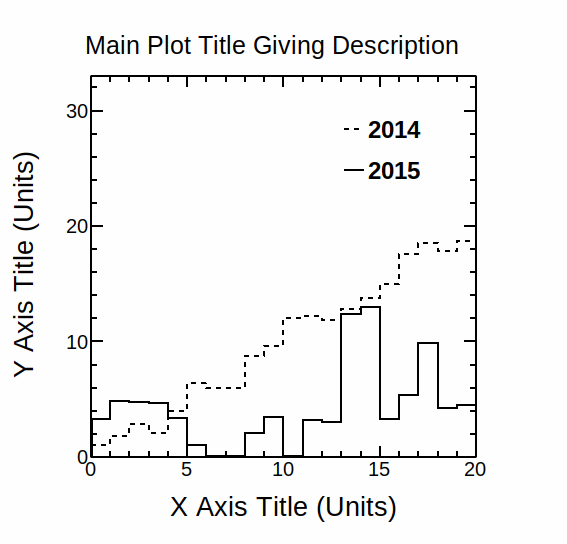
\includegraphics[scale=0.35]{pics/goodplot.png}
\end{center}
\end{frame}

\begin{frame}{Bad Plot\ldots}
\begin{center}
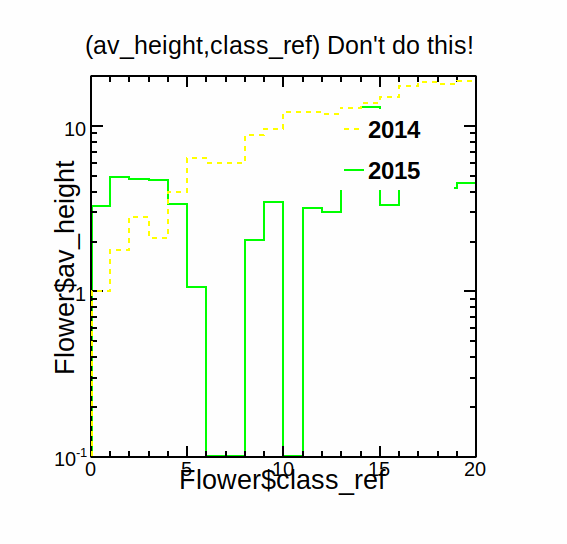
\includegraphics[scale=0.35]{pics/badplot.png}
\end{center}
\end{frame}

\begin{frame}{Assignments}
Will involve making descriptive plots for one of the R example data sets.  The details of the assignment will be given during the class.  You will be given some specific plots to make to gain familiarity with the plotting functions in R.

\end{frame}


\begin{frame}{Optional Prep}

If you are not already familiar with R then I recommend you familiarize yourself with the basics before the start of the course.  You can find some introductory material free online, I suggest working through this tutorial:

\begin{itemize}
\item https://www.nceas.ucsb.edu/files/scicomp/\\
Dloads/RProgramming/\\
BestFirstRTutorial.pdf
\end{itemize}

\noindent There are also lots of screen-casts available on YouTube, for example this series:

\begin{itemize}
\item https://www.youtube.com/watch?v=UYclmg1\_KLk
\end{itemize}


\end{frame}


\begin{frame}{Working with built in R data}

Display available data sets: \texttt{data()}

\vspace{5mm}

Once you chose one you can get help, to find its structure: \texttt{str(<data>)} and its description: \texttt{help(<data>)}.


\vspace{5mm}

You can use the \texttt{help()} function in general to see documentation
\end{frame}


\begin{frame}{Basic Plotting}

Two options you will most commonly use, I think are \texttt{hist()} and \texttt{plot()}.

\vspace{5mm}

Also see the package ggplot2: http://docs.ggplot2.org/current/


\end{frame}

\begin{frame}{Accessing Data Frames}

To begin with look at what variables you have: \texttt{str(<dataframe>)}

\vspace{5mm}

To see elements: \texttt{head(<dataframe>)}, or matrix-like access e.g. show all columns first five elements: \texttt{dataframe[1:5,]}

\vspace{5mm}

Get the content of each row by variable name: \texttt{dataframe\$variable}


\end{frame}


\begin{frame}{Problem 1: Irises}
Use the built in data frame ``iris''.  For all of the plots, make sure that you have human-readable titles and clear labelling (i.~e.~ no variable names please)

\begin{enumerate}
\item Use help(iris) to understand what variables there are - make sure you know what they all mean.
\item Make a histogram (hist) with 20 bins of petal width for the Iris Setosa.
\item Make a scatterplot (tip: try ggplot2 ggplot) of sepal length vs petal length.  Show each of the three species of Iris on the same plot with a coloured legend to separate them.
\item Make a scatterplot of sepal length vs sepal width for all Irises whose petal width is greater than 1.5.
\item Make one more plot that shows something interesting about the inter-species differences of the Irises.
\end{enumerate}


\end{frame}



%%%%%%%%%%%%% backup slides %%%%%%%%%%%%%%%%%%%%%%%%

\appendix
\newcounter{finalframe}
\setcounter{finalframe}{\value{framenumber}}

\begin{frame}{Backup Slides}
\end{frame}




\setcounter{framenumber}{\value{finalframe}}

\end{document}
